\documentclass{article}

\usepackage[utf8]{inputenc}
\usepackage[left=1.5in,right=1.5in,bottom=1in]{geometry}
\setlength\parindent{0pt}
\setlength{\parskip}{1em}
\setcounter{secnumdepth}{0}
\usepackage{outlines}
\usepackage{graphicx}
\graphicspath{ {imgs} }
\usepackage{hyperref}
\usepackage{color,soul}

\newcommand{\alignedmarginpar}[1]{%
        \marginpar{\raggedright\small #1}
    }

\title{Urban Social Geography - Summarised Notes}
\author{Carla Hyenne }

\begin{document}

\maketitle

\tableofcontents

\pagebreak

\pagebreak\section{Urban Geographical Traditions}

\textbf{Globalised urbanisation}: urbanisation is a global phenomenon. It is also unequal across the world (eg. Asia dominates economic growth and urbanisation). The `urban age' frame can be criticised:\alignedmarginpar{Brenner and Schmid, 2014} measurements depend on diverging national definitions, and it is a chaotic abstraction that does not neatly overlay cities in a spatial sense.\alignedmarginpar{Urban vs. Rural}

\textbf{The urban}: a distinctive way of life, which can take place in the city but also outside (suburbs, rural, slums). It epitomises a particular society (capitalist, industrial, fordist, modern, classist, etc.). It projects symbolic power, notably by means of its built environment.

\textbf{The city}: the material built environment. Has a complex division of labour, with increasing efficiency and surplus, but also inequalities. It projects symbolic power\alignedmarginpar{Skyscrapers (Dubai, NYC); CCTV tower (Beijing)}, and has physical and administrative boundaries. The `non-city' is hard to define, because it's hard to know where the city ends: the `rural', the peripheries, can have elements of the city.

\textbf{Urbanisation}: the process of becoming urban. It is a demographic process, whereby cities gain more and varied residents, with increasing density. It entails a globalisation of urban economic, political and cultural influence. It considers how space is organised through processes of uneven development.

\textbf{Geography}: the social and physical processes within the context of space. There are multiple concepts of space: \textbf{territory}, the boundaries and sovereignty of a space\alignedmarginpar{Brussels capital}; \textbf{scale}, the sensitivity of processes; \textbf{network}, hubs and leaks beyond the territory, towards micro-networks; and \textbf{place}, the attachement of meaning and sentiment to a space.

\textbf{Critical geography}:\alignedmarginpar{Jonas et al., Sayer, Brenner and Schmid} epistemological rules of thumb include: acknowledging that there is no universal theory of anything; knowing every theory has birthmarks, ie. is situated in time and space, and reflecting on the birthmarks is necessary to be critical\alignedmarginpar{provincialisation}; asking whether theories can be used across contexts; engaging in pluralism to allow inter-theoretical conversation and comparison.

\textbf{Materialist approaches to geography}: concerned with the distribution and social-justice, and agenda-setting.

\textbf{Humanist approaches to geography}: about the experienced city, issues of representation and discourse, uses qualitative methods, gives a voice.

\begin{center}
	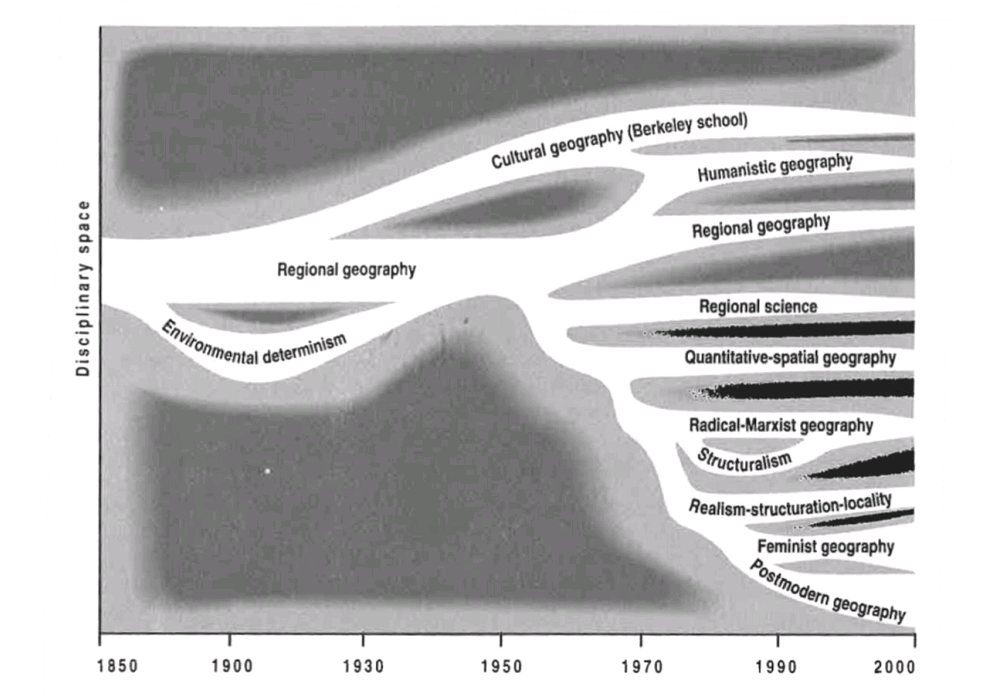
\includegraphics[width=23em]{geography_approaches.png}
\end{center}


\pagebreak\section{Theories of World-City Formation}

\textbf{}

\textbf{}

\textbf{}

\textbf{}

\textbf{}

\textbf{}

\textbf{}

\textbf{}

\textbf{}

\pagebreak\section{Polarisation in World/Global Cities}

\textbf{}

\textbf{}

\textbf{}

\textbf{}

\textbf{}

\textbf{}

\textbf{}

\textbf{}

\textbf{}

\pagebreak\section{Urban Segregation: Patterns and Causes}

\textbf{}

\textbf{}

\textbf{}

\textbf{}

\textbf{}

\textbf{}

\textbf{}

\textbf{}

\textbf{}

\pagebreak\section{Neighbourhood Effects and Living with Diversity}

\textbf{}

\textbf{}

\textbf{}

\textbf{}

\textbf{}

\textbf{}

\textbf{}

\textbf{}

\textbf{}

\pagebreak\section{Cultures of Urban Research}

\textbf{}

\textbf{}

\textbf{}

\textbf{}

\textbf{}

\textbf{}

\textbf{}

\textbf{}

\textbf{}

\pagebreak\section{Urban Cultures}

\textbf{}

\textbf{}

\textbf{}

\textbf{}

\textbf{}

\textbf{}

\textbf{}

\textbf{}

\textbf{}

\pagebreak\section{Transport and Cities: a Historical Hegemony}

\textbf{}

\textbf{}

\textbf{}

\textbf{}

\textbf{}

\textbf{}

\textbf{}

\textbf{}

\textbf{}

\pagebreak\section{Critical Perspective on Urban Transport}

\textbf{}

\textbf{}

\textbf{}

\textbf{}

\textbf{}

\textbf{}

\textbf{}

\textbf{}

\textbf{}

\end{document}
